\input{~/macro.tex}
% itemizeの変更
\renewcommand{\labelitemii}{$\circ$}
\renewcommand{\labelitemiii}{$\triangleright$}
\title{プラズマ中の波動}
\author{20B01392 松本侑真}
\date{\today}
\begin{document}
\maketitle
\begin{abstract}

\end{abstract}
\tableofcontents
\newpage

\section{概要}
プラズマ中の波動は、外部磁場$\bm{B}_0$が印加されている場合とそうでない場合などで沢山の種類に分類される。まずはプラズマ波の一覧を列挙する:
\begin{itemize}
	\item 縦波($\bm{k}\varParallel \bm{E}$):{\color{red}荷電粒子の密度擾乱}が伝播する。
	      したがって、{\color{red}Poisson方程式}(高周波振動の場合)、{\color{red}プラズマ流体運動方程式}などから分散関係を求める。
	      \begin{itemize}
		      \item $\bm{B}_0 = 0$
		            \begin{itemize}
			            \item 電子プラズマ波
			                  \begin{itemize}
				                  \item 高周波の電子による振動
			                  \end{itemize}
			            \item イオン音波
			                  \begin{itemize}
				                  \item 低周波のイオンによる振動
			                  \end{itemize}
		            \end{itemize}
		      \item $\bm{B}_0 \neq 0$(縦波であるため$\bm{B}_0\perp\bm{k}$しか考えられない。)
		            \begin{itemize}
			            \item 高域混成振動
			                  \begin{itemize}
				                  \item 背景磁場に垂直$\theta=\SI{90}{\deg}$な電子プラズマ振動であり、サイクロトロン運動とプラズマ振動の重ね合わせで書ける。
			                  \end{itemize}
			            \item 静電イオンサイクロトロン波
			                  \begin{itemize}
				                  \item $\theta\approx \SI{90}{\deg}$のイオン音波であり、横波成分を少し含んでいる場合。磁力線に垂直な方向の運動は高域混成振動と同じようにサイクロトロン運動の影響を受ける。
			                  \end{itemize}
			            \item 低域混成振動
			                  \begin{itemize}
				                  \item 厳密に$\theta = \SI{90}{\deg}$のイオン音波であり、電子、イオンのサイクロトロン運動の重ね合わせで特徴付けられる。
			                  \end{itemize}
		            \end{itemize}
	      \end{itemize}
	\item 横波($\bm{k}\perp \bm{E}$):{\color{red}荷電粒子の運動と自己無撞着に生成される電磁波}が伝播する。
	      したがって、{\color{red}誘導電磁場に関するMaxwell方程式}、{\color{red}プラズマ流体運動方程式}などから分散関係を求める。
	      \begin{itemize}
		      \item $\bm{B}_0 = 0$
		            \begin{itemize}
			            \item プラズマ周波数$\omega_P$を遮断周波数とした$\omega > \omega_P$の通常の電磁波
		            \end{itemize}
		      \item $\bm{B}_0 \neq 0 \wedge \bm{k}\perp \bm{B}_0$
		            \begin{itemize}
			            \item $\bm{E}_1 \varParallel \bm{B}_0$:正常波(O波)
			            \item $\bm{E}_1 \perp \bm{B}_0$:異常波(X波)
			            \item 磁気音波(低周波のイオン電磁波)
		            \end{itemize}
		      \item $\bm{B}_0 \neq 0 \wedge \bm{k}\varParallel \bm{B}_0$
		            \begin{itemize}
			            \item R波とL波である円偏光の重ね合わせの電磁波
			                  \begin{itemize}
				                  \item R波は電子のサイクロトロン運動と同じ方向に偏光し、L波はイオンのサイクロトロン運動と同じ方向に偏光する。
			                  \end{itemize}
			            \item Alfven波(低周波のイオン電磁波)
		            \end{itemize}
	      \end{itemize}
\end{itemize}


\subsection{CGS単位系}
教科書の単位系では、SI単位系における$\varepsilon_0,\,\mu_0$に対して
\begin{align}
	\varepsilon_0 & \to \frac{1}{4\pi} \\
	\mu_0         & \to 4\pi
\end{align}
としている。

\newpage
\section{流体としてのプラズマの解析方法}
プラズマが流体みなせるための条件は
\begin{equation}
	\text{イオンや電子の平均自由行程}\ll\text{プラズマサイズ}
\end{equation}
が満たされることである。プラズマ中で荷電粒子が十分に衝突を繰り返し、Maxwell分布での平衡状態を達成することで温度が定義される。
\subsection{理想流体としてのプラズマの運動方程式}
単一荷電粒子の運動方程式は以下で与えられた:
\begin{equation}
	m\dv{\bm{v}(t)}{t} = q\qty{\bm{E} + \bm{v}\cross\bm{B}}\;。
\end{equation}
まず、衝突や熱運動がないと仮定する。このとき、流体要素中のすべての粒子は一緒に動き、粒子の平均速度$\bm{u}$は個々の粒子の速度$\bm{v}$に等しい。
したがって、流体の方程式は密度$n$をかけることによって得られる:
\begin{equation}
	mn\dv{\bm{u}(t)}{t} = qn\qty{\bm{E} + \bm{u}\cross\bm{B}}\;。
\end{equation}
しかし、このままでは扱いにくい。なぜなら、左辺の時間微分は粒子とともに動いている座標系(Lagrange座標系)で行わねばならないからだ。
この座標系では微小な流体要素の挙動のみを追うことができる。そのため、空間に固定された座標系(Euler座標系)に変換し、プラズマ全体の集団的挙動を解析できるようにする。
すなわち、あるEuler座標系からの位置ベクトル$\bm{x}$を用いて、プラズマの速度ベクトルの位置依存性を考慮する:
\begin{equation}
	\dv{\bm{u}(\bm{x},\,t)}{t} = \pdv{\bm{u}}{t} + \pdv{\bm{u}}{x_i}\dot{x}_i = \pdv{\bm{u}}{t} + \qty(\dot{\bm{x}}\vdot\grad)\bm{u}\;。
\end{equation}
ここで、固定された座標系から見たプラズマの位置ベクトルの時間変化$\dot{\bm{x}}$は流体の移動速度$\bm{u}$に他ならず、プラズマの運動方程式は以下のように記述される:
\begin{equation}
	mn\qty[\pdv{\bm{u}}{t} + \qty(\bm{u}\vdot\grad)\bm{u}] = qn\qty{\bm{E} + \bm{u}\cross\bm{B}}\;。
	\label{eq:ideal_eq}
\end{equation}
なお、左辺第二項は対流項と呼ばれるものである。

\subsection{流体に作用するマクロな力を考慮したプラズマの運動方程式}
熱運動や衝突を考慮しない式\eqref{eq:ideal_eq}で表される運動方程式では、流体にかかるマクロな力を考慮していない。流体全体の運動量変化を考えることで、マクロな力が加わった運動方程式が導出される。
まずは、簡単のために$x$方向の圧力変化を考える。粒子は微小時間$\varDelta t$の間に平均速度$\ev{v_x}$で$\varDelta x$の距離を進むとする。

$x = x_0$が中心であり、体積$\varDelta x\varDelta y\varDelta z$の流体要素に流入する運動量$P_+$は
\begin{equation}
	P_+ = \qty[\qty(\varDelta n\ev{v_x}\varDelta y\varDelta z) m\ev{v_x}]_{x_0-\varDelta x}\varDelta t
\end{equation}
と表される。ここで、$\varDelta n$は平均速度$\ev{v_x}$を持って流体要素に流入してくる粒子数であり、$\varDelta n = n/2$の関係がある。
なお、圧力が定義できているということは、粒子の速度分布はMaxwell分布になっていることを用いた。流体要素から流出する運動量$P_-$は
\begin{equation}
	P_- = \qty[\qty(\varDelta n\ev{v_x}\varDelta y\varDelta z) m\ev{v_x}]_{x_0}\varDelta t
\end{equation}
と表される。したがって、流体要素中の運動量変化は逆方向に進む粒子も考慮して、
\begin{equation}
	\frac{\varDelta P}{\varDelta t} = 2\frac{P_+ - P_-}{\varDelta t} =\varDelta y\varDelta z\frac{\qty[mn\ev{v_x^2}]_{x_0-\varDelta x}-\qty[mn\ev{v_x^2}]_{x_0}}{\varDelta t}
\end{equation}
と表される。$\varDelta t\to 0$の極限を取ると、
\begin{equation}
	\pdv{P}{t} = -m\pdv{x}\qty(n\ev{v_x^2})\varDelta x\varDelta y\varDelta z
\end{equation}
となる。これが流体自身の正味の圧力変化と等しくなるため、
\begin{equation}
	\pdv{t}(nmu_x)\varDelta x\varDelta y\varDelta z = -m\pdv{x}\qty(n\ev{v_x^2})\varDelta x\varDelta y\varDelta z
	\label{eq:P_henka}
\end{equation}
が成立する。ここで、粒子の速度を流体速度$u_x$と熱速度$v_{xT}$に分離する:
\begin{equation}
	v_x = u_x + v_{xT},\quad \ev{u_x} = u_x,\quad \ev{v_{xT}} = 0,\quad\frac{1}{2}m\ev{v_{xT}^2} = \frac{1}{2}k_\text{B}T\;。
\end{equation}
このとき、式\eqref{eq:P_henka}は

\begin{gather}
	\pdv{t}(mnu_x)  = -m\pdv{x}\qty[n\ev{u_x^2 + 2u_xv_{xT} + v_{xT}^2}] = -m\pdv{x}\qty[n\qty(u_x^2 + \frac{k_\text{B}T}{m})] \\
	\therefore\; mn\pdv{u_x}{t} + mu_x\pdv{n}{t} = -mu_x\pdv{x}(nu_x) - mnu_x\pdv{u_x}{x} - \pdv{x}\qty(nk_{\text{B}}T)
\end{gather}
と計算できる。\footnote{$nu_x^2 = (nu_x)\vdot u_x$とみなして積の微分法を用いた。}
また、左辺が質量保存則
\begin{equation}
	\pdv{n}{t} + \pdv{x}(nu_x) = 0
\end{equation}
を用いて、流体の圧力を$P = nk_{\text{B}}T$と置くと、最終的に
\begin{equation}
	mn\pdv{u_x}{t} = - mnu_x\pdv{u_x}{x} - \pdv{P}{x}
\end{equation}
となる。したがって、$y,\,z$方向でも同様の議論が成立し、理想的な場合の運動方程式と合わせて
\begin{equation}
	mn\qty[\pdv{\bm{u}}{t} + \qty(\bm{u}\vdot\grad)\bm{u}] = qn\qty{\bm{E} + \bm{u}\cross\bm{B}} - \grad{P}
\end{equation}
となる。

\subsection{流体プラズマを記述する方程式群}
\subsubsection{運動方程式}
\begin{equation}
	mn\qty[\pdv{\bm{u}}{t} + \qty(\bm{u}\vdot\grad)\bm{u}] = qn\qty{\bm{E} + \bm{u}\cross\bm{B}} - \grad{P}
\end{equation}
\subsubsection{Maxwell方程式}
電荷密度$\sigma  = n_iq_i + n_eq_e$、電流密度$\bm{j} = n_iq_i\bm{v}_i + n_eq_e\bm{v}_e$とおける:
\begin{align}
	\div{\bm{E}}     & = 4\pi\qty(n_iq_i + n_eq_e)                                 \\
	\curl{\bm{E}}    & = -\dot{\bm{B}}                                             \\
	\div{\bm{B}}     & = 0                                                         \\
	c^2\curl{\bm{B}} & = 4\pi\qty(n_iq_i\bm{v}_i + n_eq_e\bm{v}_e)  + \dot{\bm{E}}
\end{align}

\subsubsection{連続の式}
体積$V$中の粒子の総数$N$は$V$を囲む表面$S$を横切る正味の粒子の流束がある場合にのみ変化する。粒子の流束密度は$n\bm{u}$であるため、Stokesの定理により、
\begin{equation}
	\pdv{N}{t} = \int_V\pdv{n}{t}dV = -\oint_S (n\bm{u})\vdot d\bm{S} = -\int_V \div\qty(n\bm{u})dV
\end{equation}
が任意の$V$で成立する。したがって、連続の式は以下のようになる:
\begin{equation}
	\pdv{n}{t} + \div{(n\bm{u})} = 0\;。
\end{equation}

\subsubsection{状態方程式}
圧力$p$と粒子数密度$n$を関係付ける熱力学の状態方程式を扱う:
\begin{equation}
	p = C\rho^\gamma\;。
\end{equation}
ここで、$C$は定数で$\gamma$は比熱比$C_p/C_V$である。したがって、
\begin{equation}
	\frac{\grad{p}}{p} = \gamma\frac{\grad{n}}{n}
\end{equation}
となり、等温圧縮では
\begin{equation}
	\grad{p} = \grad\qty(nk_{\text{B}}T) = k_{\text{B}}T\grad{n}
\end{equation}
が成立するため、明らかに$\gamma=1$となる。断熱圧縮に対しては、自由度$N$に対して
\begin{equation}
	\gamma = (2+N)/N
\end{equation}
が成立する。
\subsection{外部磁場に対する流体ドリフトについて}
\subsubsection{外部磁場に垂直な流体ドリフト}
流体要素はたくさんの粒子から成っているため、個々の粒子の旋回中心が外部磁場$\bm{B}$に垂直な方向にドリフトをすれば、流体も$\bm{B}$に垂直な方向にドリフトされることが期待される。
しかし、実際は$\grad{\bm{B}}$ドリフトは流体中に存在せず、圧力勾配が存在する場合には流体全体のドリフト運動が生じることを示す。

まず、プラズマ中の粒子の運動方程式
\begin{equation}
	mn\qty[\pdv{\bm{v}}{t} + \qty(\bm{v}\vdot\grad)\bm{v}] = qn\qty{\bm{E} + \bm{v}\cross\bm{B}} - \grad{P}
\end{equation}
において、$\bm{v} = e^{i(\bm{k}\vdot\bm{r} - wt)}$とおく。また、磁場に垂直な成分$\bm{v}_{\perp}$の運動を考えることにする。サイクロトロン角周波数$\omega_c = qB/m$を用いると、
\begin{equation}
	\qty|\frac{mn\pdv*{\bm{v}_\perp}{t}}{qn\bm{v}_{\perp}B}| = \qty|\frac{m\omega}{qB}| \approx \frac{\omega}{\omega_c}
\end{equation}
となるため、サイクロトロン運動の時間スケールより遅いドリフトであれば$\pdv*{\bm{v}_{\perp}}{t}$は無視できる。
また、後にわかることであるが、対流項は$\qty(\bm{v}_{\perp}\vdot\grad)\bm{v}_{\perp} = 0$となるため、無視して計算を行う。
$\bm{B}$との外積を作ることで、運動方程式は以下のように変形できる:
\begin{equation}
	\begin{aligned}
		0 & = qn\qty[\bm{E}\cross\bm{B} + \qty(\bm{v}_{\perp}\cross\bm{B})\cross\bm{B}] - \grad{P}\cross\bm{B}                 \\
		  & = qn\qty[\bm{E}\cross\bm{B} + \bm{B}\qty(\bm{v}_{\perp}\vdot\bm{B}) - \bm{v}_{\perp}B^2] - \grad{P}\cross\bm{B}\;。
	\end{aligned}
\end{equation}
したがって、
\begin{equation}
	\bm{v}_{\perp} = \frac{\bm{E}\cross\bm{B}}{B^2} - \frac{\grad P\cross\bm{B}}{qnB^2} \eqqcolon \bm{v}_\text{E} + \bm{v}_\text{D}
\end{equation}
と求まる。ここで、
\begin{equation}
	\bm{v}_\text{E} = \frac{\bm{E}\cross\bm{B}}{B^2}\qquad\text{$\bm{E}\cross\bm{B}$ドリフト}
\end{equation}
\begin{equation}
	\bm{v}_\text{D} =  - \frac{\grad P\cross\bm{B}}{qnB^2} \qquad\text{反磁性ドリフト}
\end{equation}
である。反磁性ドリフトによってプラズマが反磁性の性質を持つことを図解する。図\ref{fig:entyu}は、円柱プラズマ内に磁場が印加されており、中心軸方向に圧力勾配が存在する場合を表している。
\begin{figure}[H]
	\centering
	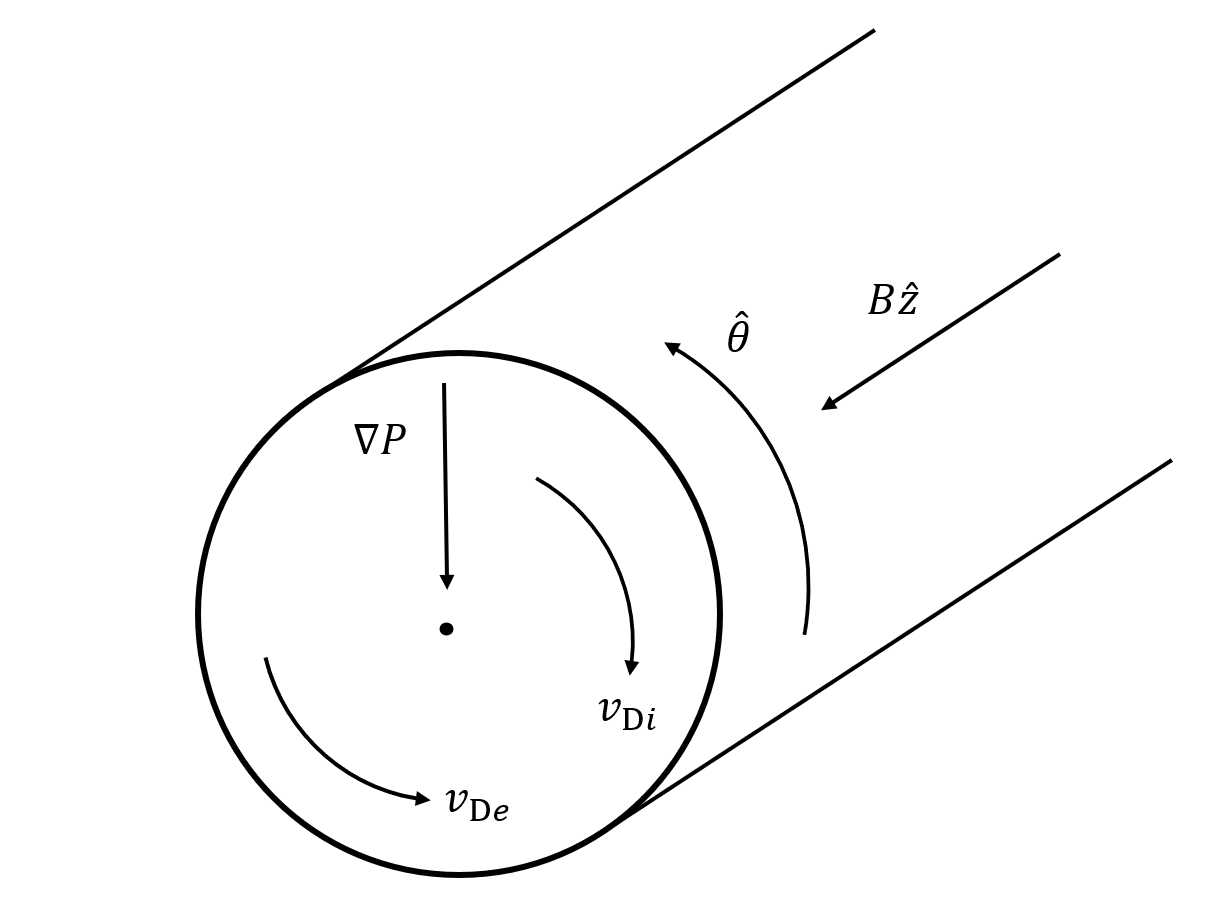
\includegraphics[width=0.7\linewidth]{entyuu_plasma.png}
	\caption{円柱プラズマ内の反磁性ドリフト}
	\label{fig:entyu}
\end{figure}
$\grad{P}\propto -\hat{r},\,\bm{B}\propto \hat{z}$であるため、$\bm{v}_{\text{D}}\propto -\hat{\theta}$となる。
すなわち、イオンの反磁性ドリフト、電子の反磁性ドリフトそれぞれが外部磁場$\bm{B}$を打ち消す方向の円電流を生むことがわかる。
そのため、プラズマ内に同じ方向の電流$\bm{j}_{\text{D}}$が生じることがわかる。その値はプラズマ近似$n_i=n_e=n$の元で
\begin{equation}
	\bm{j}_{\text{D}} = qn(\bm{v}_{\text{D}i} - \bm{v}_{\text{D}e}) = \qty(k_{\text{B}}T_i + k_{\text{B}}T_e)\frac{\bm{B}\cross\grad{n}}{B^2}
\end{equation}
である。
最後に、対流項が磁場に垂直な成分を持たないことを示す。
\begin{equation}
	\bm{v}\vdot\grad =
	\begin{pmatrix}
		v_r & v_\theta & v_z
	\end{pmatrix}
	\begin{pmatrix}
		\pdv{r}                 \\
		\frac{1}{r}\pdv{\theta} \\
		\pdv{z}
	\end{pmatrix}
\end{equation}
であることと、$\bm{v}_{\text{D}} = v(r)\hat{\theta}$と表されることより、
\begin{equation}
	\qty(\bm{v}_{\text{D}}\vdot\grad)\bm{v}_{\text{D}} = \qty(v(r)\frac{1}{r}\pdv{\theta})v(r)\hat{\theta} = 0
\end{equation}
となる。

\subsubsection{外部磁場に平行な流体ドリフト}
流体の運動方程式の$z$成分は
\begin{equation}
	mn\qty[\pdv{v_z}{t} + (\bm{v}\vdot\grad)v_z] = qnE_z - \pdv{p}{z}
\end{equation}
である。対流項は時間微分項に比べて無視できることが多い。$p=Cn^\gamma$を代入すると、
\begin{equation}
	\pdv{v_z}{t} = \frac{qE_z}{m} - \frac{\gamma k_{\text{B}}T}{mn}\pdv{n}{z}
\end{equation}
となる。$m\to 0$の極限(イオンに比べて電子の方が質量が小さいため、電子に対する運動方程式を考えていることになる。)をとると、
\begin{equation}
	qE_z = \frac{\gamma{}k_{\text{B}}T}{n}\pdv{n}{z}
\end{equation}
となる。$q=-e,\,\bm{E} = -\grad{\phi}$を用いて両辺を積分すると、
\begin{equation}
	n=n_0\exp\qty(\frac{e\phi}{k_{\text{B}}T})
\end{equation}
と求まる。すなわち、プラズマ中の電子(外部磁場に平行な成分)はBoltzmann分布をしていることになる。
イオンに比べて電子の質量は非常に小さいため、電子は大きな移動度を持つ。
電場によって速やかに高エネルギーに加速されるため、このような分布を取る。

\subsection{プラズマ近似}
電子の慣性項が無視できるとき、電子運動は低周波でなければならない。
逆に、高周波の運動を考える際には電子の慣性項が無視できなくなる:$m_e\pdv{\bm{v}_e}{t} \neq 0\;。$

電子が低周波運動を行っているとき、プラズマでは普通$n_i = n_e,\,\div{\bm{E}} \neq 0$を同時に満たされると仮定することが可能である。これをプラズマ近似と呼ぶ。
プラズマ近似が成立している際に$\bm{E}$を求めるためにPoisson方程式
\begin{equation}
	\div{\bm{E}} = 4\pi e(n_i-n_e)
\end{equation}
を用いることができないことに注意する必要がある。
また、電子が高周波で運動している場合にプラズマ近似ができないのは、イオンの質量が大きいため電子の運動に追従することができなくなり、電子とイオンの密度に差が生じてしまうからである。


\section{方程式の線形化と単一モード解析}
いろんな種類の波に対する共通の考え方が方程式の線形化と単一モード解析である。
単一モード解析とは、各周波数$\omega$と波数$k$を用いて、物理量$\bm{A}$が
\begin{equation}
	\bm{A}(\bm{r},\,t) = \exp\qty{i\qty(\bm{k}\vdot\bm{r} - \omega{}t)}
\end{equation}
と表されることを元にして分散関係を導出することである。
方程式の線形化とは、全ての物理量を平衡成分と摂動成分(それぞれ添え字に0と1を)に分けることである。
そして、その摂動成分がどのような関数系になっているかを導出するということである。
また、摂動成分はその1次項までで近似する。
\subsection{プラズマ振動}
例として、電子に対する方程式群
\begin{gather}
	mn_e\qty[\pdv{\bm{v}_e}{t} + \qty(\bm{v}_e\vdot\grad)\bm{v}_e]  = -en_e\bm{E} \\
	\pdv{n_e}{t} + \div(n_e\bm{v}_e)                                = 0           \\
	\div{\bm{E}}                                                    = -4\pi{}en_e
\end{gather}
を線形化してみる。これは、プラズマ中の電子がイオンの一様なバックグラウンドから変位したときに、電子自身が生む電場によって元の位置に戻す復元力が働く場合を考えている。
すなわち、プラズマの中性を保とうとする方向の電場が自動的に生じている。これを解くと、電子は{\color{red}プラズマ周波数}と呼ばれる特性周波数で平衡位置を行き来して振動する。
その振動は非常に早く、イオンは電子の振動に追従できずに動かないと考える。最も簡単な場合として、
\begin{itemize}
	\item 外部磁場は存在しない。
	\item 熱運動はしていない。
	\item イオンは空間中に一様に分布し固定されている。
	\item プラズマは無限に大きい。
	\item 電子の運動は$\hat{\bm{x}}$方向のみである。
\end{itemize}
という仮定をおいて考える。
$\bm{E} = \bm{E}_0 + \bm{E}_1$として、$\bm{E}_1$成分について線形化すると、
\begin{gather}
	m\pdv{\bm{v}_1}{t}                                                    = -e\bm{E}_1 \\
	\pdv{n_{e1}}{t} + n_{e0}\div{\bm{v}_{e1}} + \bm{v}_{e0}\grad{n_{e0}}  = 0          \\
	\div{\bm{E}_1} = -4\pi e n_{e1}
\end{gather}
と1次の摂動で書ける。すべての摂動を$\exp\qty{i(\bm{k}\vdot\bm{r} - \omega{}t)}$として、
$\bm{v}_{e1} = v_1\hat{\bm{x}},\,\bm{E}_1 = E_1\hat{\bm{x}}$として解くと、線形化した方程式は
\begin{align}
	-im\omega{}v_1   & = -eE_1           \label{eq:1} \\
	-i\omega{}n_{e1} & = -n_{e0}ikv_{e1} \label{eq:2} \\
	ikE_1            & = -4\pi{}en_{e1} \label{eq:3}
\end{align}
となる。これはイオンについても同様に成立する。上の2式から
\begin{equation}
	n_{e1} = \frac{k}{\omega}n_{e0}v_{e1} = \frac{k}{\omega}n_{e0}\qty(\frac{-ie}{m\omega})E_1
\end{equation}
となり、これを最後の式に代入すると、
\begin{equation}
	\omega^2 E_1 = \frac{4\pi{}n_{e0}e^2}{m}E_1 = \omega^2_{pe}E_1
\end{equation}
となり、$\omega_{pe}$を電子プラズマ周波数と呼ぶ。質量$M$のイオンの寄与まで考えると、
\begin{equation}
	\omega^2E_1 =  4\pi{}n_{e0}e^2\qty(\frac{1}{m} + \frac{1}{M})E_1
\end{equation}
となり、
\begin{equation}
	\omega_{pi} = \sqrt{\frac{4\pi{}n_{e0}e^2}{M}}
\end{equation}
をイオンプラズマ周波数と呼ぶ。

\newpage
\section{縦波}
\subsection{電子プラズマ波}
電子のプラズマ振動が熱運動によって伝播する波が電子プラズマ波である。熱運動を考慮するために断熱変化による圧力項
\begin{equation}
	P_e = C\rho_e^\gamma,\gamma=3
\end{equation}
を付与する。(一次元運動を考えるため$\gamma=3$となる。)このとき、両辺の対数微分と状態方程式$P_e = n_ek_{\text{B}}T_e$を用いると
\begin{equation}
	\grad{P_e} = 3k_{\text{B}}T_e\grad{n_e} = 3k_{\text{B}}T_e\grad(n_{e0} + n_{e1}) = 3k_{\text{B}}T_e\pdv{n_{e1}}{x}\hat{\bm{x}}
\end{equation}
となる。したがって、線運動方程式
\begin{equation}
	mn_e\pdv{\bm{v}_e}{t}= -en_e\bm{E} - \grad{P_e}
\end{equation}
を線形化すると、$x$方向は
\begin{equation}
	mn_{e0}\pdv{v_1}{t} = -en_{e0}E_1 - 3k_{\text{B}}T_e\pdv{n_{e1}}{x}
\end{equation}
となる。\footnote{摂動の2次以上の項は無視している。}
単一モード解析を行うと、式\eqref{eq:1}、式\eqref{eq:2}、式\eqref{eq:3}と同じようにして
\begin{align}
	-im\omega{}n_{e0}v_1 & = -en_0E_1  -3k_{\text{B}}T_eikn_{e1} \\
	-i\omega{}n_{e1}     & = -n_{e0}ikv_{e1}                     \\
	ikE_1                & = -4\pi{}en_{e1}
\end{align}
を組み合わせる。$n_{e1} = (k/{\omega})n_{e0}v_1$
を用いながら下2式を一番上の式に代入して、
\begin{equation}
	im\omega{}n_{e0}v_1  = en_{e0}i\frac{4\pi{}e}{k}\frac{k}{\omega}n_{e0}v_1 + 3k_{\text{B}}T_eik\frac{k}{\omega}n_{e0}v_1
\end{equation}
つまり、
\begin{equation}
	\omega^2v_1 = \qty(\frac{4\pi{}n_{e0}e^2}{m} + \frac{3k_{\text{B}}T_e}{m}k^2)v_1
\end{equation}
を得る。熱速度$v_{\text{th}}^2$を$v_{\text{th}}^2 = 2k_{\text{B}}T_e/m$で定義すると、分散関係は以下のようになる:
\begin{equation}
	\omega^2 = \omega^2_{pe} + \frac{3}{2}k^2v^2_{\text{th}}\;。
\end{equation}

電子プラズマ波の位相速度と群速度は、$2\omega{}\dd{\omega} = 3kv^2_{\text{th}}\dd{k}$より
\begin{align}
	\text{位相速度}\quad{}v^2_{\phi} & \coloneqq \frac{\omega^2}{k^2} = \qty(\frac{\omega_{pe}}{k})^2 + \frac{3}{2}v^2_{\text{th}} \to \frac{3}{2}v^2_{\text{th}}\quad(k\to\infty)\;, \\
	\text{群速度}\quad{}v_g         & \coloneqq \pdv{\omega}{k} = \frac{3}{2}\frac{k}{\omega}v^2_{\text{th}} = \frac{3}{2}\frac{v^2_{\text{th}}}{v_{\phi}}
	\begin{cases}
		\to\sqrt{\frac{3}{2}}v_{\text{th}} & \quad(k\to\infty) \\
		< v_{\text{th}}                    & \quad(k\to 0)
	\end{cases} \quad\text{(情報の伝達速度)}
\end{align}
となる。すなわち、
\begin{itemize}
	\item $k\to\infty$のとき、波の情報は熱運動で伝わる。これは、通常の流体中の微小擾乱が音波の速度で伝わるのと同じである。\footnote{\url{https://takun-physics.net/2738/}を参考。}
	\item $k\to 0$のとき、位相速度$v_{\phi}$は熱速度$v_{\text{th}}$より大きくても、波の情報は熱速度よりゆっくりと伝わる。熱速度は、縦波の代表的な位相速度である。(横波は光速$c$である。)
\end{itemize}



\subsection{イオン音波}
イオン音波を導出するためには、イオンの慣性項が重要であるため、低周波振動を考えることになる。
そのため、プラズマ近似が成立しており、プラズマ振動や電子プラズマ波の場合のように、Poisson方程式を用いることができない。
その代わりに連続の式を用いることで、イオン衝突の振動であるイオン音波を導出することができる。

磁場のないときのイオン流体の方程式は、電場が静電場であると仮定し、状態方程式を用いると
\begin{align}
	Mn_{i}\qty[\pdv{\bm{v}_{i}}{t} + ({\bm{v}_{i}}\vdot\grad)\bm{v}_{i}] = en\bm{E} - \grad{P} = -en_i\grad{\phi} - \gamma_ik_{\text{B}}T_i\grad{n_i}
\end{align}
となる。これを1次の摂動までで線形化すると
\begin{equation}
	Mn_{i0}(-i\omega)v_{i1} = -en_{i0}ik\phi_1 - \gamma_ik_{\text{B}}T_iikn_{i1}
	\label{eq:ion_undou}
\end{equation}
となる。なお、圧力勾配や密度勾配にはイオンの寄与のみを考えた。\footnote{これの妥当性がよくわからないと思ったが、$\gamma_e=1$の話をしているところで解決済み?}
ここで、$\bm{B}=\bm{0}$であるため、電子の密度分布がBoltzmann分布になっていることより、
\begin{equation}
	n_e = n_i = n_0\exp\qty(\frac{e\phi_1}{k_{\text{B}}T_e}) = n_0\qty(1 + \frac{e\phi_1}{k_{\text{B}}T_e}) = n_0 + n_1
\end{equation}
となる。なお、$n_0$は平衡プラズマの密度を表しており、電子とイオンがともにBoltzmann分布をしているため$\bm{E}_0=\bm{0}$と仮定することができる。
そのため$\phi_0 = 0$と置いた。

また、イオンの連続の式
\begin{equation}
	\pdv{n_i}{t} + \div{\qty(n_i\bm{v}_i)} = 0
\end{equation}
を線形化すると
\begin{equation}
	i\omega{}n_{i1} = ikn_{i0}v_{i1}
\end{equation}
となるため運動方程式は、$n_{i0} = n_0$とおいて
\begin{equation}
	Mn_0\omega{}v_{i1} = en_0k\frac{k_{\text{B}}T_e}{en_0}\frac{kn_0v_{i1}}{\omega} + \gamma_ik_{\text{B}}T_ik\frac{kn_0v_{i1}}{\omega}
\end{equation}
となる。したがって、
\begin{equation}
	\omega^2 = k^2\qty(\frac{k_{\text{B}}T_e}{M} + \frac{\gamma_ik_{\text{B}}T_i}{M}) \iff \frac{\omega}{k} = \sqrt{\frac{k_{\text{B}}T_e + \gamma_ik_{\text{B}}T_i}{M}} \coloneqq v_s
\end{equation}
と分散関係が求まる。なお、位相速度と群速度は同じ値であり、$v_s$はプラズマ中の音速を表す。

なお、今仮定している縦波の平面波では、イオンは1次元の圧縮を受けることになるため、$\gamma_i = 3$となる。
電子はこの波と比べて非常に速く動くため、温度が均一になりやすく等温であると考えて良い。そのため圧力勾配の式において電子の寄与を考えておらず、$\gamma_e=1$が省略されているとみなせる。
さもなければ$v_s$中で$\gamma_ek_{\text{B}}T_e$と補正されることになる。

また、$T_i = 0$でも$T_e > 0$であればイオン音波は伝搬することがわかる。
イオン自身は運動エネルギーを持たないものの、電子がBoltzmann分布を形成する際の摂動によって電場を形成することで、それに引っ張られる運動が生じているのである。
\subsection{プラズマ近似を用いないイオン音波}
イオン音波を導く際にプラズマ近似を用いた。今回はプラズマ近似を用いずにPoisson方程式からイオン音波を導きその誤差を見る:
\begin{equation}
	\div{\bm{E}_1} = k^2\phi_1 = 4\pi{}e\qty(n_{i1}-n_{e1}),\quad n_{e1} = n_0\frac{e\phi_1}{k_{\text{B}}T}\;。
\end{equation}
これらより、
\begin{equation}
	\phi_1\qty(k^2+\frac{4\pi{}n_0e^2}{k_{\text{B}}T}) = 4\pi{}en_{e1} \iff \phi_1\qty(k^2+\frac{1}{\lambda_{D}^2}) = 4\pi{}en_{e1}
\end{equation}
を得る。イオン密度$n_{i1}$は線形化したイオンの連続の式から得られる:
\begin{equation}
	\omega{}n_{i1} = kn_{i0}v_{i1}\;。
\end{equation}
これらをイオンの運動方程式\eqref{eq:ion_undou}に代入すると、
\begin{equation}
	Mn_{i0}\omega{}v_{i1} = en_{i0}k\frac{4\pi{}e\lambda_{D}^2}{k^2\lambda_{D}^2 + 1}\frac{kn_{i0}v_{i1}}{\omega} + \gamma_ik_{\text{B}}T_ik\frac{kn_{i0}v_{i1}}{\omega}
\end{equation}
となる。したがって、
\begin{equation}
	\omega^2 = \frac{k^2}{M}\qty(\frac{4\pi{}n_{i0}e^2\lambda_D^2}{k^2\lambda_D^2 + 1} + \gamma_ik_{\text{B}}T_i)
	\iff \frac{\omega}{k} = \sqrt{\frac{k_{\text{B}}T_e}{M}\frac{1}{k^2\lambda_{D}^2 + 1} + \frac{\gamma_ik_{\text{B}}T_i}{M}}
\end{equation}
と分散関係が求まる。これは、分母を除けば先に得られた式と一致する。そのためプラズマ近似を仮定した場合、その誤差は$k^2\lambda_D^2 = (2\pi\lambda_D/\lambda)^2$ほどの誤差を与える。
そのため、Debye長$\lambda_D$より長波長の擾乱に対してはプラズマ近似を適用して良い。一方で$k^2\lambda_D^2\gg 1$の短波長極限の擾乱のとき、
\begin{equation}
	\omega^2 = k^2\frac{4\pi{}n_{i0}e^2}{Mk^2} = \frac{4\pi{}n_{i0}e^2}{M} = \Omega_{pi}^2 \quad(T_i\to 0)
\end{equation}
となる。すなわち、高い周波数においてはイオン音波の周波数はイオンプラズマ周波数で一定値となる。
\subsubsection{電子プラズマ波とイオン音波の相補的関係}
電子プラズマ波とイオン音波の分散関係と速度をまとめる。
\begin{align}
	\text{電子プラズマ波:} &
	\begin{dcases}
		\text{分散関係}\quad \omega^2  = \omega_{pe}^2 + \frac{3}{2}k^2v_{\text{th}}^2\to \omega_{pe}^2                                    & \quad(k\to 0)     \\
		\text{位相速度} = \frac{\omega^2}{k^2} = \qty(\frac{\omega_{pe}}{k})^2 + \frac{3}{2}v^2_{\text{th}} \to \frac{3}{2}v^2_{\text{th}} & \quad(k\to\infty) \\
		\text{群速度} = \pdv{\omega}{k} = \frac{3}{2}\frac{k}{\omega}v^2_{\text{th}}
		= \frac{3}{2}\frac{v^2_{\text{th}}}{v_{\phi}}\to\sqrt{\frac{3}{2}}v_{\text{th}}                                                & \quad(k\to\infty)
	\end{dcases} \\
	\text{イオン音波:}   &
	\begin{dcases}
		\text{分散関係}\quad\omega^2 = \frac{k^2}{M}\qty(\frac{4\pi{}n_{i0}e^2\lambda_D^2}{k^2\lambda_D^2 + 1} + \gamma_ik_{\text{B}}T_i) \to \Omega_{pi}^2 & \quad(k\to\infty) \\
		\text{位相速度} = \text{群速度} = \sqrt{\frac{k_{\text{B}}T_e + \gamma_ik_{\text{B}}T_i}{M}}                                                           & \quad(k\to0)
	\end{dcases}
\end{align}
すなわち、
\begin{itemize}
	\item 長波長極限:電子プラズマ波は分散関係が一定値、イオン音波は速度が一定値
	\item 短波長極限:電子プラズマ波は速度が一定値、イオン音波は分散関係が一定値
\end{itemize}
となる。

\subsection{高域混成振動:背景磁場に垂直な電子プラズマ振動}
以下は外部磁場$\bm{B}_0$が存在する場合の縦波である。まずは、$\bm{B}_0$に垂直な電子振動を考える。
なお、垂直、平行は摂動を受けない磁場$\bm{B}_0$に対する$\bm{k}$の方向を表す。
縦、横は摂動している電場$\bm{E}_1$に対する$\bm{k}$の方向を示す。
また、摂動している磁場$\bm{B}_1 = \bm{0}$ならば静電的な波動であり、そうでなければ電磁的な波動である。これは、
\begin{equation}
	\curl{\bm{E}_1} = -\dot{\bm{B}}_1 \iff \bm{k}\cross\bm{E}_1 = \omega\bm{B}_1
\end{equation}
に起因している。例えば縦波($\bm{k}\varParallel\bm{E}_1$)であれば摂動磁場がなくなり、波動は静電波になる。

高域混成振動では以下の2つを仮定している。すなわち、電子の高周波振動を考えることになる。(Poisson方程式を用いることができる。)
\begin{itemize}
	\item イオンは空間的に不動で一様
	\item 熱運動$k_{\text{B}}T_e$は$0$であるため、圧力項は存在しない。
\end{itemize}
今は縦波を考えているため、座標軸を$\bm{k} = k\hat{\bm{x}},\,\bm{E}_1 = E_1\hat{\bm{x}},\,\bm{B}_0 = B_0\hat{\bm{z}}$と取ることができる。また、電子の運動は以下の方程式群で記述される:
\begin{align}
	m\pdv{v_{e1}}{t}                          & = -e\qty(\bm{E}_1 + \bm{v}_{e1}\cross\bm{B}_0)\;, \\
	\pdv{n_{e1}}{t} + \div(n_{e0}\bm{v}_{e1}) & = 0\;,                                            \\
	\div{\bm{E}_1}                            & = -4\pi{}en_{e1}\;。
\end{align}
運動方程式を成分ごとに表して線形化すると
\begin{align}
	-i\omega{}mv_{x} & = -eE_1 - ev_yB_0 \\
	-i\omega{}mv_y   & = ev_xB_0         \\
	-i\omega{}mv_z   & = 0
\end{align}
となる。$v_y$を消去すると、$\omega_c = eB_0/m$を用いて
\begin{equation}
	i\omega{}mv_{x} = eE_1 + e\frac{iev_xB_0}{\omega{}m}B_0 \iff v_x = \frac{eE_1/im\omega}{1 - \omega^2_c/\omega^2}
\end{equation}
となる。サイクロトロン共鳴$\omega=\omega_c$では電場と$v_x$の位相が常に一致し、常に$v_x$方向の加速を促すために$v_x$は無限大へと発散してしまう。
さらに、分散関係を求めるために他2式を用いると、
\begin{equation}
	ikn_{e0}\frac{eE_1/im\omega}{1-\omega^2_c/\omega^2} = -i\omega\frac{ikE_1}{4\pi{}e} \iff\omega^2 \qty(1-\frac{\omega^2_c}{\omega^2}) = \frac{4\pi{}n_0e^2}{m} = \omega^2_{pe}
\end{equation}
を得る。すなわち、
\begin{equation}
	\omega^2 = \omega^2_{pe} + \omega^2_c \coloneqq \omega_{\text{UH}}^2\quad\text{(Upper Hybrid oscillation)}
\end{equation}
と計算できる。つまり、背景磁場$\bm{B}_0$に沿う運動は、電子の変位に起因する復元力で通常のプラズマ振動を行い、磁場を横切る運動はサイクロトロン角周波数で磁力線を横切る運動を行うと解釈できる。

\newpage

\subsection{静電イオンサイクロトロン波:背景磁場に「ほぼ」垂直なイオン音波}
次に背景磁場が存在する場合のイオン音波について考える。高域混成振動と同様に、背景磁場の効果を見たいため、磁場に垂直な成分を考える。
また、$\bm{k}\vdot\bm{B}_0 = kB_0\cos\theta$と置いたときの$\theta$が厳密に$\pi/2$である場合とそうでない場合で電子の運動が大きく異なるため、
まずは「ほぼ」垂直であるとして考える。なお、イオンの運動に関しては大きな違いは生じない。電子が$\bm{B}_0$に対する運動としては
\begin{itemize}
	\item $\bm{B}_0$に垂直な方向:サイクロトロン運動によるLarmor半径が小さいために異なる磁力線へと移ることができない。
	\item $\bm{B}_0$に平行な方向:$\theta\neq 0$であるため、磁力線に沿って運動することでイオン音波の定密度面間を運動することができる。
	      すなわち、平行な方向にはDebye遮蔽を形成する。(図\ref{fig:hobo90}参考)
\end{itemize}
イオンは慣性が大きいため、電子のように異なる波面に移ることができず、イオンの運動に関しての波数は$\bm{k} = k\hat{\bm{x}}$とみなして良い。
また、以下では簡単のために$k_{\text{B}}T_i = 0,\,k_{\text{B}}T_e\neq 0$とする。$T_i=0$でもイオン音波は存在し、重要な物理が見られるため問題ない。
さらに、$\bm{k}\cross\bm{E} = 0$の静電波を仮定し、$\bm{E} = -\grad\phi$とする。
\begin{figure}[H]
	\centering
	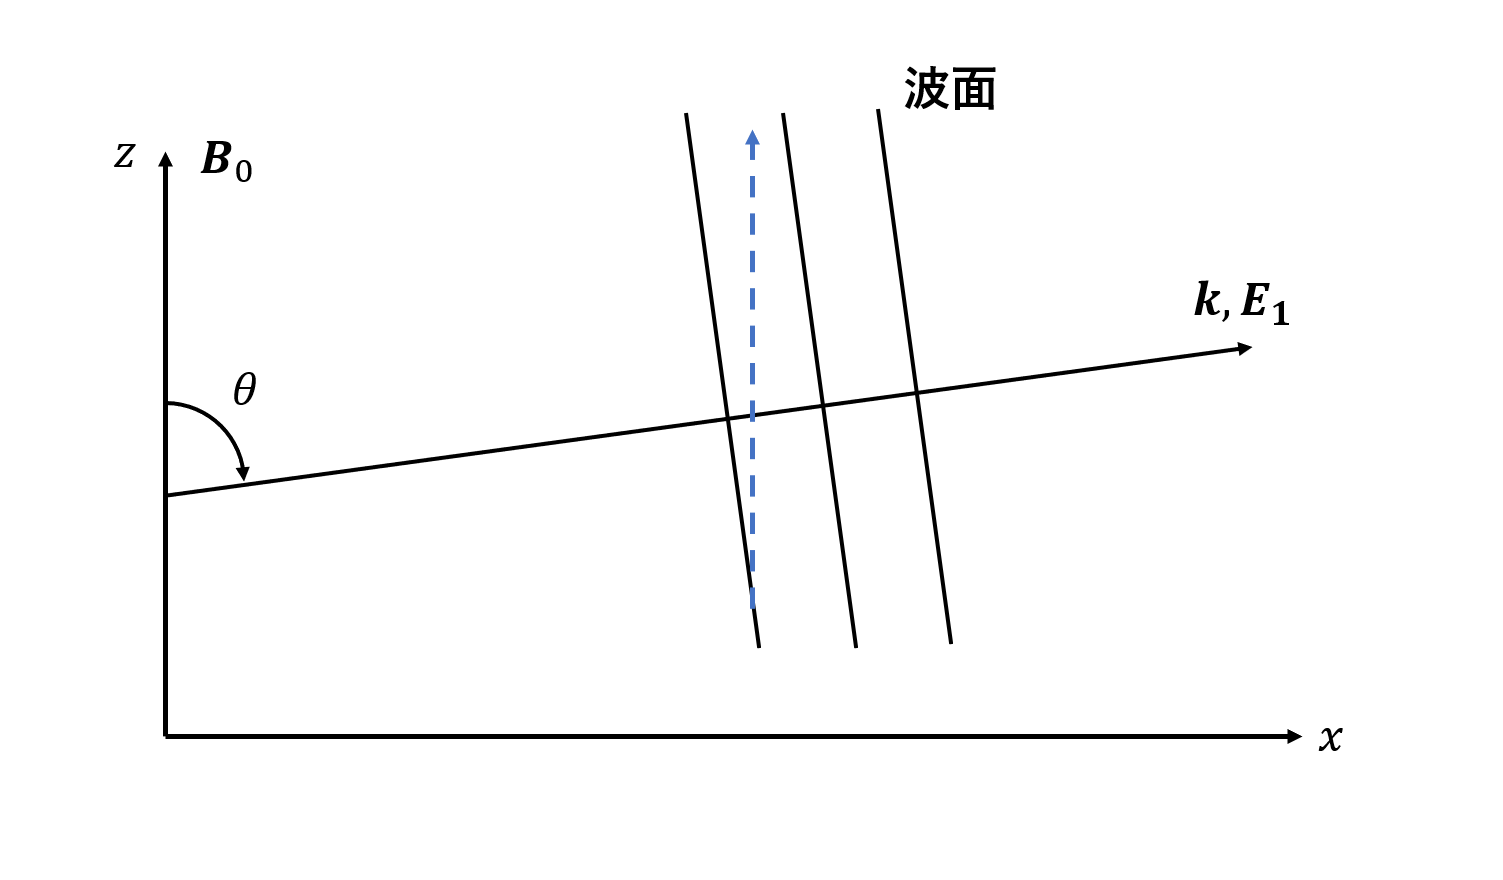
\includegraphics[width=0.8\linewidth]{hobo90.png}
	\caption{$\bm{B}_0$に対してほぼ垂直な静電イオンサイクロトロン波}
	\label{fig:hobo90}
\end{figure}

このとき、イオンの運動方程式は
\begin{equation}
	M\pdv{v_{i1}}{t} = -e\grad{\phi_1} + e\bm{v}_{i1}\cross\bm{B}_0
\end{equation}
となる。Poisson方程式と連続の式を含めて単一モード解析を行って成分ごとに分けると、(イオンの波動は$x$方向のみであることに注意して)
\begin{align}
	-i\omega{}Mv_{ix}                & = -eik\phi_1 + ev_{iy}B_0 \\
	-i\omega{}Mv_{iy}                & = -ev_{ix}B_0             \\
	-ik\phi_1                        & = 4\pi{}en_{i1}           \\
	-i\omega{}n_{i1} +n_{i0}ikv_{ix} & = 0
\end{align}
となる。上の2式から、イオンサイクロトロン周波数を$\Omega_{c} = eB/M$とおくと
\begin{equation}
	\omega{}Mv_{ix} = ek\phi_1 + e\frac{ev_{ix}B_0}{\omega{}M}B_0 \implies v_{ix} = \frac{ek}{\omega{}M}\phi_1\qty(1-\frac{\Omega^2_c}{\omega^2})^{-1}
\end{equation}
を得る。さらに、電子は$\bm{B}_0$方向に動けるため、電子についてBoltzmann分布が成立していると仮定して良い。さらに、電子は低周波振動を考えているためプラズマ近似が成立し、
\begin{equation}
	n_{i1} = n_{e0}\frac{e\phi_1}{k_{\text{B}}T_e}
\end{equation}
となる。そのため、残りの方程式を用いると
\begin{equation}
	\qty(1-\frac{\Omega^2_c}{\omega^2})v_{ix} = \frac{ek}{\omega{}M}\frac{k_{\text{B}}T_e}{en_{e0}}\frac{n_{i0}k}{\omega}v_{ix}
	\implies \omega^2 = \Omega^2_c + k^2\frac{k_{\text{B}}T_e}{M} = \Omega^2_c + k^2v^2_s
\end{equation}
と分散関係が求まる。この波は高域混成振動の物理と似ていることがわかる。イオン音波のときに導いたように、イオンは音波型の振動を行うが、外部磁場によるLorentz力でサイクロトロン運動の復元力が働く。
また、電子によるDebye遮蔽が形成されている場合は、外部磁場の影響を考えなくて済むため、通常のイオン音波の分散関係$\omega^2 = k^2v^2_s$が適用できる。

\subsection{低域混成振動:厳密に垂直なイオン音波}
次に、厳密に$\theta=\SI{90}{deg}$であるときのイオン音波を考える。このとき、電子の密度分布はBoltzmann分布を形成できず、イオンと同じ運動を行う。
すなわち、イオンの結果において$e\to{}-e,\,M\to{}m,\,\Omega_c\to{}-\omega_c$と置き換えるだけで良い。そのため、
\begin{equation}
	v_{ex} = -\frac{ek}{\omega{}m}\phi_1\qty(1-\frac{\omega_c^2}{\omega^2})^{-1},\,n_{e1} = n_0\frac{k}{\omega}v_{e1}
\end{equation}
が成立する。プラズマ近似が成立しているため、$n_{i1} = n_{e1}\iff v_{i1} = v_{e1}$とすると、
\begin{equation}
	M\qty(1-\frac{\Omega^2_c}{\omega^2}) = -m\qty(1 - \frac{\omega^2_c}{\omega^2}) \implies \omega^2(M+m) = m\omega^2_c + M\Omega^2_c = e^2B^2\qty(\frac{1}{m} + \frac{1}{M})
\end{equation}
となる。したがって、
\begin{equation}
	\omega^2 = \frac{e^2B^2}{Mm} = \Omega_c\omega_c \iff \omega = \qty(\Omega_c\omega_c)^{1/2}\eqqcolon \omega_1
\end{equation}
と分散関係が求まり、$\omega_1$を低域混成周波数と呼ぶ。これは$\theta=\pi/2$が正確に成立している際の静電イオン振動の周波数である。

\newpage
\section{横波}
\subsection{外部磁場がない場合}
$\bm{B}=\bm{0}$のときの横波であるため、$\bm{j}_1$をプラズマ電流として、Maxwell方程式から導かれる以下の方程式を解く:
\begin{align}
	\curl(\curl{\bm{E}}_1)   & =  \grad(\div{\bm{E}}_1) - \laplacian\bm{E}_1 = -\curl\dot{\bm{B}}_1\;, \\
	c^2\curl{\dot{\bm{B}}_1} & = 4\pi\pdv{\bm{j}_1}{t} + \ddot{\bm{E}}_1\;。
\end{align}
単一モード解析を用いると、横波では$\div{\bm{E}}_1 = \bm{k}\vdot\bm{E}_1 = 0$であることより
\begin{equation}
	c^2k^2\bm{E}_1 = -\qty(-4\pi{}i\omega{}\bm{j}_1 - \omega^2\bm{E}_1) \implies (\omega^2 - c^2k^2)\bm{E}_1 = -4\pi{}i\omega\bm{j}_1
\end{equation}
となる。なお、今の状況では以下の仮定を置いている:
\begin{itemize}
	\item 高周波振動を考えている。(イオンは不動である。)
	\item 電子の熱運動は考えていない。($\grad{P}$が発生して縦波を考えてしまうことになるため。)
\end{itemize}

プラズマ電子電流と電子の運動方程式はそれぞれ
\begin{align}
	\bm{j}_1              & = -n_0e\bm{v}_{e1}                                  \\
	m\pdv{\bm{v}_{e1}}{t} & = -e\bm{E}_1 \iff -im\omega\bm{v}_{e1} = -e\bm{E}_1
\end{align}
より
\begin{equation}
	\bm{j}_1 = \frac{in_0e^2}{m\omega}\bm{E}_1
\end{equation}
であるため、これを先ほどの式に代入すると、
\begin{equation}
	(\omega^2 - c^2k^2)\bm{E}_1 = \frac{4\pi n_0e^2}{m}\bm{E}_1 = \omega^2_{pe}\bm{E}_1 \iff \omega^2 = \omega^2_{pe} + c^2k^2
\end{equation}
と分散関係が求まる。位相速度、群速度、屈折率は以下のように計算される:
\begin{align}
	\text{位相速度}\quad{}v^2_{\phi} & \coloneqq \frac{\omega^2}{k^2} = c^2 + \frac{\omega^2_{pe}}{k^2} > c^2\;,                                                  \\
	\text{群速度}\quad{}v_g         & \coloneqq \pdv{\omega}{k} = \frac{c^2k}{\sqrt{\omega^2_{pe} + c^2k^2}} = \frac{c^2}{v_{\phi}} < c \quad\text{(情報の伝達速度)}\;, \\
	\text{屈折率}\quad{}N^2         & \coloneqq \frac{c^2}{v^2_{\phi}} = \frac{c^2k^2}{\omega^2} = 1 - \frac{\omega^2_{pe}}{\omega^2} < 1\;。
\end{align}
すなわち、プラズマ中では荷電粒子の塊が存在しているはずであるが、真空よりも屈折率が低いという奇妙な結果が生じている。また、以下のような事実がわかる:
\begin{itemize}
	\item プラズマの電子密度が大きくなると、$\omega_{pe}\propto \sqrt{n}$であるため屈折率は小さくなっていく。
	\item $\omega=\omega_{pe}$となるプラズマ密度$n_e = \frac{m\omega^2_{pe}}{4\pi e^2}$(臨界密度)で電磁波が遮断される。プラズマは$\omega > \omega_{pe}$を満たす高周波の波しか通さない。{\color{red}物理的にはなぜ?}
	      \begin{itemize}
		      \item 通信衛星を考えると、電離層に遮断されないように高周波帯域を用いる方が良い。
		      \item 地上での通信では電離層で反射させるために低周波帯域を用いる方が良い。
	      \end{itemize}
\end{itemize}
\subsection{正常波:電場と背景磁場が平行な場合}
次に、$\bm{B}_0$が存在する場合のときの電磁波の伝播を考える。最初に$\bm{k}\perp\bm{B}_0$の波動について考察する。
この場合、$\bm{E}_1\varParallel \bm{B}_0$と$\bm{E}_1\perp \bm{B}_0$の2通りの自由度が存在する。正常波(O波)は前者の場合であるため、
$\bm{B}_0 = B_0\hat{\bm{z}},\,\bm{E}_1 = E_1\hat{\bm{z}},\,\bm{k} = k\hat{\bm{x}}$と書ける。波が従う方程式は磁場のない場合と同じであり、
\begin{equation}
	(\omega^2-c^2k^2)\bm{E}_1 = -4\pi{}i\omega{}\bm{j}_1 = 4\pi{}in_0e\omega\bm{v}_{e1}
\end{equation}
である。$\bm{E}_1 \propto\hat{\bm{z}}$であるため、電子速度の$z$成分について考えれば良い。$z$方向の電子の運動方程式は
\begin{equation}
	m\pdv{v_{1z}}{t} = -eE_{1z}
\end{equation}
であり、磁場によるLorentz力は働かない。したがって、
\begin{equation}
	(\omega^2 - c^2k^2)E_{1z} = 4\pi{}in_0e\omega\frac{eE_{1z}}{im\omega} = \omega^2_pE_{1z}
\end{equation}
を得る。これは$\bm{B}_0 = \bm{0}$の場合の電磁波と全く同じ分散関係であり、そのために正常波と呼ばれる。

\subsection{異常波:電場と背景磁場が垂直な場合}
次に、$\bm{E}_1\perp\bm{B}_0$の波動を考える。この場合、電子の運動は背景磁場によるLorentz力が働くため、分散関係が変化する。
座標軸は$\bm{B}_0 = B_0\hat{\bm{z}},\,\bm{E}_1 = E_1\hat{\bm{y}},\,\bm{k} = k\hat{\bm{x}}$と取る。
しかし、実際にはLorentz力により電子の運動は$\hat{\bm{x}}$方向にも生じる。そのため、厳密な横波を形成することができず、縦波成分も存在する。
このことを考慮するために、$\bm{E}_1 = E_x\hat{\bm{x}} + E_y\hat{\bm{y}}$として取り扱う必要がある。
このとき、モード解析によって線形化した電子の運動方程式は
\begin{equation}
	-im\omega\bm{v}_{e1} = -e\qty(\bm{E}_1 + \bm{v}_{e1}\cross\bm{B}_0)
\end{equation}
となる。$x,\,y$成分について書き下すと、
\begin{align}
	v_x & = \frac{-ie}{m\omega}\qty(E_x + v_yB_0) \\
	v_y & = \frac{-ie}{m\omega}\qty(E_y - v_xB_0)
\end{align}
となる。これを解くと
\begin{equation}
	\begin{dcases}
		v_x & = \frac{e}{m\omega}\qty(-iE_x -\frac{\omega_c}{\omega}E_y + \frac{\omega_cB_0}{\omega}v_x)  \\
		v_y & = \frac{e}{m\omega}\qty(-iE_y + \frac{\omega_c}{\omega}E_x - \frac{\omega_cB_0}{\omega}v_y)
	\end{dcases}\implies
	\begin{dcases}
		v_x & = \frac{e}{m\omega}\qty(-iE_x - \frac{\omega_c}{\omega}E_y)\qty(1-\frac{\omega^2_c}{\omega^2})^{-1} \\
		v_y & = \frac{e}{m\omega}\qty(-iE_y + \frac{\omega_c}{\omega}E_x)\qty(1-\frac{\omega^2_c}{\omega^2})^{-1}
	\end{dcases}
\end{equation}
となる。また、波の方程式は$\div{\bm{E}_1} = i\bm{k}\vdot\bm{E}_1 = ikE_x$であり、$\grad{ikE_x} = ik\grad{E_x} = -kE_x\bm{k}$となることから、
\begin{equation}
	(\omega^2 - c^2k^2)\bm{E}_1 + c^2kE_x\bm{k} = -4\pi{}i\omega\bm{j}_1 = 4\pi{}in_0\omega{}e\bm{v}_{e1}
	\label{eq:ijouha}
\end{equation}
となる。これを成分にわけて$v_x,\,v_y$の表式を代入すると、
\begin{align}
	\omega^2E_x            & = -4\pi{}in_0\omega{}e\frac{e}{m\omega}\qty(iE_x + \frac{\omega_c}{\omega}E_y)\qty(1-\frac{\omega^2_c}{\omega^2})^{-1} \\
	(\omega^2 - c^2k^2)E_y & = -4\pi{}in_0\omega{}e\frac{e}{m\omega}\qty(iE_y- \frac{\omega_c}{\omega}E_x)\qty(1-\frac{\omega^2_c}{\omega^2})^{-1}
\end{align}
となる。$\omega^2_{ep} = 4\pi{}n_0e^2/m$を用いて変形すると、
\begin{align}
	\qty[\omega^2\qty(1-\frac{\omega_c^2}{\omega^2}) - \omega^2_{pe}]E_x + i\frac{\omega^2_{pe}\omega_c}{\omega}E_y            & = 0 \\
	-i\frac{\omega^2_{pe}\omega_c}{\omega}E_x +\qty[(\omega^2 - c^2k^2)\qty(1-\frac{\omega^2_c}{\omega^2}) - \omega^2_{pe}]E_y & = 0
\end{align}
つまり、
\begin{equation}
	\begin{pmatrix}
		\omega^2\qty(1-{\omega_c^2}/{\omega^2}) - \omega^2_{pe} & i{\omega^2_{pe}\omega_c}/{\omega}                                  \\
		-i{\omega^2_{pe}\omega_c}/{\omega}                      & (\omega^2 - c^2k^2)\qty(1-{\omega^2_c}/{\omega^2}) - \omega^2_{pe}
	\end{pmatrix}
	\begin{pmatrix}
		E_x \\ E_y
	\end{pmatrix} = 0
\end{equation}
となる。$\bm{E}\neq\bm{0}$より行列式を解くと、$\omega_{\text{UH}} = \omega^2_c + \omega^2_{pe}$を用いると、
\begin{equation}
	\begin{vmatrix}
		\omega^2 - \omega^2_{\text{UH}}    & i{\omega^2_{pe}\omega_c}/{\omega}                                       \\
		-i{\omega^2_{pe}\omega_c}/{\omega} & \omega^2 - \omega^2_{\text{UH}} - c^2k^2\qty(1-{\omega^2_c}/{\omega^2})
	\end{vmatrix} = 0
\end{equation}
を解くことになり、
\begin{equation}
	(\omega^2-\omega^2_{\text{UH}})\qty[\omega^2-\omega^2_{\text{UH}} - c^2k^2\qty(1-\frac{\omega^2_c}{\omega^2})] = \qty(\frac{\omega^2_{pe}\omega_c}{\omega})^2
\end{equation}
と変形できる。これは
\begin{equation}
	\frac{c^2k^2}{\omega^2}\qty(\omega^2-\omega^2_c) = \omega^2-\omega^2_{\text{UH}} - \frac{(\omega^2_{pe}\omega_c/\omega)^2/(\omega^2-\omega^2_{\text{UH}})}{\omega^2-\omega^2_{\text{UH}}}
\end{equation}
となる。位相速度$v_{\phi}$を用いると$c^2k^2/\omega^2 = c^2/v^2_{\phi}$となることから、分散関係は
\begin{equation}
	\frac{c^2}{v^2_{\phi}} = \frac{\omega^2-\omega^2_{\text{UH}} - (\omega^2_{pe}\omega_c/\omega)^2/(\omega^2-\omega^2_{\text{UH}})}{\omega^2-\omega^2_c}
\end{equation}
となる。ここで、$\omega^2_{\text{UH}} = \omega^2_{pe} + \omega^2_c$と戻すと
\begin{align}
	\frac{c^2}{v^2_{\phi}} & = \frac{\omega^2 - \omega^2_{pe} - \omega^2_c - (\omega^4_{pe}\omega^2_c/\omega^2)/(\omega^2-\omega^2_{\text{UH}})}{\omega^2-\omega^2_c}                 \\
	                       & = 1-\frac{\omega^2_{pe}\qty(\omega^2-\omega^2_{pe}-\omega^2_c + \omega^2_{pe}\omega_c^2/\omega^2)}{(\omega^2-\omega^2_c)(\omega^2-\omega^2_{\text{UH}})}
	= 1-\omega^2_{pe}\frac{(\omega^2-\omega^2_c-\omega^2_{pe}\qty(1-\omega^2_{c}/\omega^2))}{(\omega^2-\omega^2_c)(\omega^2-\omega^2_{\text{UH}})}                                    \\
	                       & =1-\frac{\omega^2_{pe}}{\omega^2}\frac{(\omega^2-\omega^2_c)\qty(\omega^2-\omega^2_{pe})}{(\omega^2-\omega^2_c)(\omega^2-\omega^2_{\text{UH}})}
	= 1-\frac{\omega^2_{pe}}{\omega^2}\frac{\omega^2-\omega^2_{pe}}{\omega^2-\omega^2_{\text{UH}}}
\end{align}
と求まる。

\subsection{外部磁場と波数ベクトルが平行な場合}
次に、$\bm{B}_0=B_0\hat{\bm{z}},\,\bm{k} = k\hat{\bm{z}},\,\bm{E}_1 = E_x\hat{\bm{x}} + E_y\hat{\bm{y}}$とする。
このとき、異常波の方程式において$\bm{k}$を変更すれば良いだけであり、式\eqref{eq:ijouha}を参考にして、
\begin{align}
	(\omega^2 - c^2k^2)E_x & = \omega^2_{pe}\qty(E_x -i\frac{\omega_c}{\omega}E_y)\qty(1-\frac{\omega^2_c}{\omega^2})^{-1} \\
	(\omega^2 - c^2k^2)E_y & = \omega^2_{pe}\qty(E_y +i\frac{\omega_c}{\omega}E_x)\qty(1-\frac{\omega^2_c}{\omega^2})^{-1}
\end{align}
となる。ここで、$\alpha = \frac{\omega^2_{pe}}{1-\omega^2_c/\omega^2}$と置くと
\begin{align}
	(\omega^2 - c^2k^2 - \alpha)E_x + i\alpha\frac{\omega_{c}}{\omega}E_y & =0 \label{eq:LR1} \\
	-i\alpha\frac{\omega_{c}}{\omega}E_x + (\omega^2-c^2k^2-\alpha)E_y    & =0 \label{eq:LR2}
\end{align}
と整理できる。行列式が$0$の条件から、
\begin{equation}
	(\omega^2-c^2k^2-\alpha)^2 = \qty(\frac{\alpha\omega_{c}}{\omega})^2 \iff (\omega^2-c^2k^2-\alpha) = \pm\frac{\alpha\omega_{c}}{\omega}
\end{equation}
と2つの解が出てくる。したがって、
\begin{equation}
	\omega^2-c^2k^2 = \alpha\qty(1\pm\frac{\omega_{c}}{\omega}) = \frac{\omega_{pe}^2}{1-(\omega_c/\omega)^2}\qty(1\pm\frac{\omega_{c}}{\omega})
	= \frac{\omega_{pe}^2}{1\mp(\omega_c/\omega)^2}
\end{equation}
と計算できる。分散関係は以下のようになる:
\begin{equation}N^2 = \frac{c^2k^2}{\omega^2}=
	\begin{dcases}
		1-\frac{\omega^2_{pe}/\omega^2}{1-(\omega_c/\omega)^2} \quad\text{(R波)}\;, \\
		1-\frac{\omega^2_{pe}/\omega^2}{1+(\omega_c/\omega)^2} \quad\text{(L波)}\;。
	\end{dcases}
\end{equation}
R波とL波はそれぞれ右回り、左回り円偏光を表す。外部磁場が存在する場合の横波についてまとめると、
\begin{itemize}
	\item $\bm{B}_0 \varParallel \bm{k}$:平面偏光波である正常波($\bm{B_0}\varParallel\bm{E}_1$)と楕円偏光波である異常波($\bm{B_0}\perp\bm{E}_1$)
	\item $\bm{B}_0 \perp \bm{k}$:右回り円偏光の$R$波と左回り円偏光の$L$波の重ね合わせ
\end{itemize}
となる。
\subsubsection{$L$波と$R$波が円偏光を成すことの証明}
式\eqref{eq:LR2}に$i$をかけて式\eqref{eq:LR1}に加えると、
\begin{equation}
	\qty(\omega^2-c^2k^2-\alpha)\qty(E_x+iE_y) + \alpha\frac{\omega_c}{\omega}\qty(E_x + iE_y) = 0
\end{equation}
となる。式\eqref{eq:LR2}に$-i$をかけて式\eqref{eq:LR1}に加えると、
\begin{equation}
	\qty(\omega^2-c^2k^2-\alpha)\qty(E_x-iE_y) - \alpha\frac{\omega_c}{\omega}\qty(E_x - iE_y) = 0
\end{equation}
となる。したがって、L波とR波の分散関係を求める式は
\begin{equation}
	\begin{dcases}
		F(\omega)\qty(E_x+iE_y)=0,\wedge{}G(\omega)\qty(E_x-iE_y)=0       \\
		F(\omega) = \omega^2-c^2k^2-\alpha\qty(1-\frac{\omega_c}{\omega}) \\
		G(\omega) = \omega^2-c^2k^2 - \alpha\qty(1+\frac{\omega_c}{\omega})
	\end{dcases}
\end{equation}
と変形できる。ここで、L波は$F(\omega)=0$が成立するときであり、R波は$G(\omega)=0$が成立するときの波である。
すなわち、L波の電場は
\begin{equation}
	E_x - iE_y=0
\end{equation}
が成立している。つまり、$E_x \propto e^{-i\omega{}t},\,E_y \propto e^{-i(\omega{}t + \pi/2)}$とおくことができる。
これは、$E_y$が$E_x$より位相が$\pi/2$だけ進んでいることを意味している。$z$軸正方向から$xy$平面を見ると、$z=0$の波面は右回転していることがわかる。波動が進む方向は$z$軸正方向であるため、L波は左円偏光を表す波動である。
\begin{table}[H]
	\centering
	\caption{$E_x$と$E_y$の時間経過}
	\begin{tabular}{ccc}
		\toprule
		$\omega{}t$ & $E_x$ & $E_y$ \\
		\midrule
		$0$         & 1     & 0     \\
		$T/4$       & 0     & -1    \\
		$T/2$       & -1    & 0     \\
		$3T/4$      & 0     & 1     \\
		\bottomrule
	\end{tabular}
	\label{tab:my_label}
\end{table}







\newpage
\section{遮断周波数と共鳴周波数}
\begin{itemize}
	\item 遮断(cutoff)周波数とは、プラズマ中の屈折率$N$が$N=ck/\omega=0$となるときの周波数である。
	      \begin{itemize}
		      \item 波数$k=0$に対応し、波がプラズマ表面で反射されることを表す。
	      \end{itemize}
	\item 共鳴(resonance)周波数とは、プラズマ波の位相速度$v_{\phi}$が$v_{\phi}=\omega/k=0$となるときの周波数である。
	      \begin{itemize}
		      \item 波長$\lambda=0$に対応し、波はプラズマ中に入ることができるが伝播せずに振動することを表す。
		      \item 共鳴周波数の条件は$N\to\infty$と見ても良い。
	      \end{itemize}
\end{itemize}
\subsection{異常波について}
異常波の分散関係は
\begin{equation}
	N^2 = \frac{c^2}{v^2_{\phi}} = 1-\frac{\omega^2_{pe}}{\omega^2}\frac{\omega^2-\omega^2_{pe}}{\omega^2-\omega^2_{\text{UH}}}
	= 1-\frac{\omega^2_{pe}}{\omega^2}\frac{1}{1-\omega^2_c/(\omega^2-\omega^2_{pe})}
\end{equation}
であった。したがって、遮断周波数を与える方程式は以下のようになる:
\begin{align}
	1-\frac{\omega^2_c}{\omega^2-\omega^2_{pe}} & = \frac{\omega^2_{pe}}{\omega^2} \notag                             \\
	1-\frac{\omega^2_{pe}}{\omega^2}            & = \frac{\omega^2_c/\omega^2}{1-\qty(\omega^2_{pe}/\omega^2)} \notag \\
	\qty(1-\frac{\omega^2_{pe}}{\omega^2})^2    & = \frac{\omega^2_c}{\omega^2}                                \notag \\
	\omega^2 \mp \omega_c\omega -\omega^2_{pe}  & = 0
\end{align}
したがって、
\begin{equation}
	\omega_R = \frac{1}{2}\qty[\omega_c + \qty(\omega_c^2 + 4\omega_{pe}^2)^{1/2}],\,\omega_L =  \frac{1}{2}\qty[-\omega_c + \qty(\omega_c^2 + 4\omega_{pe}^2)^{1/2}]
\end{equation}
がそれぞれの波のカットオフ周波数である。また、共鳴周波数は
\begin{equation}
	\omega = \omega_{\text{UH}} = \sqrt{\omega^2_{pe} + \omega^2_c}
\end{equation}である。

\subsection{正常波について}
正常波の分散関係は
\begin{equation}
	\omega^2 = \omega^2_{pe} + c^2k^2
\end{equation}
であった。したがって、
\begin{equation}
	N^2 = \frac{c^2k^2}{\omega^2} = 1 - \frac{\omega^2_{pe}}{\omega^2}
\end{equation}
となる。つまり、カットオフ周波数は$\omega = \omega_{pe}$で、共鳴周波数は存在しない。

\subsection{$L$波と$R$波について}
$L$波と$R$波の分散関係は
\begin{equation}N^2 = \frac{c^2k^2}{\omega^2}=
	\begin{dcases}
		1-\frac{\omega^2_{pe}/\omega^2}{1-(\omega_c/\omega)^2} \quad\text{(R波)} \\
		1-\frac{\omega^2_{pe}/\omega^2}{1+(\omega_c/\omega)^2} \quad\text{(L波)}
	\end{dcases}
\end{equation}
であった。R波については、共鳴周波数が$\omega=\omega_c$であり、カットオフ周波数は異常波のそれと同じ方程式(符号が負の方)で与えられる。したがって、
カットオフ周波数は$\omega=\omega_R$となる。

L波については共鳴周波数が存在しない。直感的には、L波の偏光方向は電子のサイクロトロン運動と逆方向であるために共鳴しないという理解ができる。
実際にイオンの運動を考慮して方程式を解くと、共鳴周波数はイオンサイクロトロン周波数$\omega=\Omega_c$で共鳴周波数を持つ。
カットオフ周波数は$\omega=\omega_L$である。

\section{まとめ}



\end{document}